\section{Linearisierung}

\subsubsection{Repetition Tangentengleichung}

Dient als Annäherung für eindimensionale $f(x)$ in der Nähe von $x_0$ (Linearisierung): \\
$g(x) = f(x_0) + f'(x_0)(x - x_0)$




\subsection{Jacobi-Matrix}
Sozusagen wie Tangentengleichung aber für mehrere Variablen
$$\vec{y} = \vec{f}(\vec{x}) =
	\begin{pmatrix}
		y_1 = f_1(x_1, ..., x_n) \\
		\hdots                   \\
		y_m = f_m(x_1, ..., x_n) \\
	\end{pmatrix}
$$

Die Jacobi-Matrix enthält sämtliche Partielle Ableitungen 1. Ordnung von $\vec{f}$. \\
Auf jeder Spalte bleibt die funktion $f_j$ die gleiche und in den
Zeilen $x_i$ $\rightarrow$ $\dfrac{\partial f_j}{\partial x_i}$

\begingroup
\renewcommand*{\arraystretch}{1.8}
\scalemath{1.2}{
	D\vec{f}(x) =
	\begin{pmatrix}
		\dfrac{\partial f_1}{\partial x_1}(x) & \dfrac{\partial f_1}{\partial x_2}(x) & \hdots & \dfrac{\partial f_1}{\partial x_n} \\
		\dfrac{\partial f_2}{\partial x_1}(x) & \dfrac{\partial f_2}{\partial x_2}(x) & \hdots & \dfrac{\partial f_2}{\partial x_n} \\
		\vdots                                & \vdots                                & \ddots & \vdots                             \\
		\dfrac{\partial f_m}{\partial x_1}(x) & \dfrac{\partial f_m}{\partial x_2}(x) & \hdots & \dfrac{\partial f_m}{\partial x_n} \\
	\end{pmatrix}
}
\endgroup

\subsubsection{verallgemeinerte Tangentengleichung}

$$\vec{g}(\vec{x}) = \vec{f}(\vec{x}^{(0)}) + D\vec{f}(\vec{x}^{(0)}) * (\vec{x} - \vec{x}^{(0)})$$

ist eine lineare Funktion und für $\vec{x}$ in der Umgebung von
$\vec{x}^{(0)} = (x^{(0)}_1,x^{(0)}_2, ..., x^{(0)}_n)$
gilt $\vec{f}(\vec{x}) \approx \vec{g}(\vec{x})$

$Df$ entspricht der obigen Funktion zur Erzeugung einer Jacobi-Matrix.

Hochgestellte Zahlen in Klammern ($x^{(n)}$) stehen wie zuvor für eine Variable
nach $n$ Iterationsschritten.



\subsection{Tangentialebene}

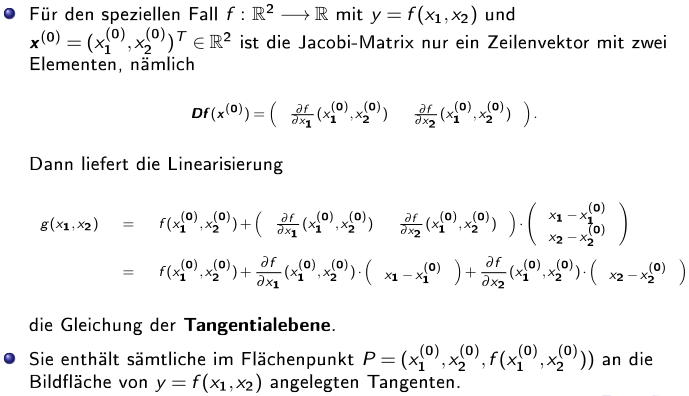
\includegraphics[width=\linewidth]{tangentialebene}


Graphische Darstellung der Fläche $x_3 = f(x_1, x_2) = x_1^2 + x_2^2$
sowie Tangentialebene durch den Flächenpunkt $(x^{(0)}_1 = 1, x^{(0)}_2 = 2, f(x^{(0)}) = 5)$


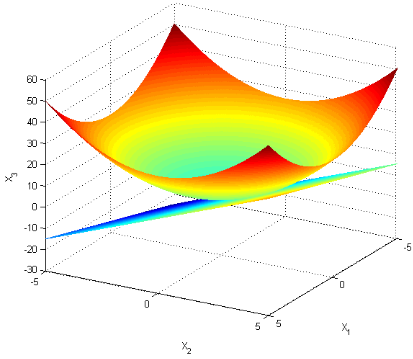
\includegraphics[scale=0.4]{tangentialebene-vis}








%TODO move
\section{Nullstellenbestimmung für nichtlineare Systeme}


\begin{itemize}
	\item Gegeben: $n \in \N$ und eine Funktion $\vec{f} : \R^n \to \R^n$
	\item Gesucht: $\vec{x} \in \R^n \quad \mathrm{mit} \quad \vec{f}(\vec{x}) = 0$
	      $$
		      \vec{f}(x_1,...,x_n) =
		      \begin{pmatrix}
			      f_1(x_1,...,x_n) \\
			      \vdots           \\
			      f_n(x_1,...,x_n) \\
		      \end{pmatrix}
		      = \vec{0}
	      $$
\end{itemize}






\subsection{Newton-Verfahren für Systeme}


\subsubsection{Herleitung}

Repetition 1-Dimensional: (nur für $f: \R \to \R$)

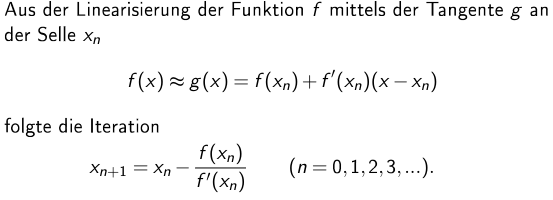
\includegraphics[scale=0.4]{newton-rep-1d}


Mit der Jacobi-Matrix $Df(x)$ kann das analog für Vektor-wertige
Funktionen $f: \R^n \to \R^n$ angewendet werden.

\begin{center}
	\scalemath{1.5}{
		$$\v x^{(n+1)} = \v x^{(n)} - (Df(\v x^{(n)}))^{-1} * \v f(\v x^{(n)})$$
	}
\end{center}


Das Inverse der Jacobi-Matrix wird aber nie berechnet sondern die obige Gleichung
via Substitution als lineares Gleichungsystem aufgefasst.

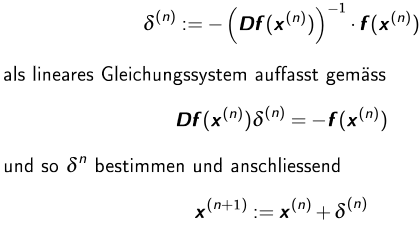
\includegraphics[scale=0.4]{newton-jacobi-subst}





\subsection{Quadratisch-konvergentes Newton-Verfahren für Systeme}
% TODO code

Gesucht: Nullstellen von $\v f : \R^n \to \R^n$ mit Startvektor $\v x^{(0)}$
Nahe der Nullstelle.\\
\textcolor{red}{es kann passieren, dass das Newton-Verfahren Statt einer Nullstelle
	ein lokales Minimum $x_{min} != 0$ findet, in diesem Fall ist $Df(x_{min})$
	aber immer nicht regulär.}

\textcolor{blue}{
	\Large{
		für $n = 0, 1,...$:
		\begin{enumerate}
			\item Berechne $\delta^{(n)}$ als Lösung des linearen Gleichungsystems
			      $$ D\v{f}(\v x^{(n)}) \delta^{(n)} = - \v f(\v x^{(n)}) $$
			\item Setze
			      $$ \v x^{(n+1)} = \v x^{(n)} + \delta^{(n)} $$
		\end{enumerate}
	}
}

\subsubsection{mögliche Abbruchkriterien}

\begin{itemize}
	\item $n \ge n_{max}, \, n_{max} \in \N$
	\item $|| x^{(n+1)} - x^{(n)} || \le \epsilon
		      \qquad \leftrightarrow \qquad || \delta^{(n)} || \le \epsilon$
	\item $|| x^{(n+1)} - x^{(n)} || \le \epsilon * || x^{(n+1)} ||$
	\item $|| \v f(x^{(n+1)}) || \le \epsilon$
\end{itemize}

\subsubsection{Konvergenz}

Das Newton-Verfahren konvergiert quadratisch für nahe genug an einer Nullstelle
$\v x$ liegende Startvektoren, wenn $D\v f(\v x)$ regulär und $\v f$ dreimal
stetig differenzierbar ist.







\subsection{Vereinfachtes Newton-Verfahren für Systeme}
% TODO code

Gesucht: Nullstellen von $\v f : \R^n \to \R^n$ mit Startvektor $\v x^{(0)}$
Nahe der Nullstelle.\\

Der Unterschied zum Quadratisch-konvergenten Newton-Verfahren liegt darin, dass
nur einmal die Jacobi-Matrix für den Startvektor berechnet werden muss (rot)
$\rightarrow$ weniger Aufwand aber konvergiert langsamer (linear).

\textcolor{blue}{
	\Large{
		für $n = 0, 1,...$:
		\begin{enumerate}
			\item Berechne $\delta^{(n)}$ als Lösung des linearen Gleichungsystems
			      $$ D\v{f}( \textcolor{red}{ \v x^{(0)} } ) \delta^{(n)} = - \v f(\v x^{(n)}) $$
			\item Setze
			      $$ \v x^{(n+1)} = \v x^{(n)} + \delta^{(n)} $$
		\end{enumerate}
	}
}



\subsection{Gedämpftes Newton-Verfahren}
% TODO code

Die Idee ist bei jedem Iterationsschritt zu überprüfen ob es sich um eine
Verbesserung handelt und falls nicht, es stattdessen mit einem gedämpften Schritt
zu versuchen.

Die gewählte Dämpfungsgrösse $k_{max}$ ist stark vom Problem abhängig.
\textcolor{PineGreen}{$k_{max} = 4$ ist ein vernünftiger Standard Wert.}


\textcolor{blue}{
	\Large{
		für $n = 0, 1,...$:
		\begin{enumerate}
			\item Berechne $\delta^{(n)}$ als Lösung des linearen Gleichungsystems
			      $$ D\v{f}(\v x^{(n)}) \delta^{(n)} = - \v f(\v x^{(n)}) $$
			\item Finde das minimale $k \in {0,1,...,k_{max}}$ mit
			      $$ || \v f(x^{(n)}) + \frac{\delta^{(n)}}{2^k} ||_2
				      < || \v f(x^{(n)}) ||_2  $$
			\item Setze (falls kein minimales $k \rightarrow k = 0$)
			      $$ \v x^{(n+1)} = \v x^{(n)} + \frac{ \delta^{(n)} }{ 2^{k} } $$
		\end{enumerate}
	}
}

